
\documentclass[11pt]{article} 
\usepackage{styles/preamble_diss}

\title{Strategic fitting and spectral line assignment in rotational molecular spectroscopy}
\author{Kirill Borisov}

\begin{document}

\begin{titlepage}
\maketitle
\end{titlepage}

\tableofcontents
\newpage

\section{Introduction}


%In this chapter, procedures for analysis and fitting rotational molecular spectra analysis are described along with tools and methods for this task. That leads to a discussion of new approaches with a focus on automation (reducing human effort). Examples are given with spectra of three molecules with increasing complexity of their spectra: OCS, vinyl cyanide (acrylonitrilie) and thiazole. Among them OCS is the simplest case, a linear top; the other two molecules are asymmetric tops: vinyl cyanide has a slightly crinkled carbon chain with a cyano (CN) group at the end and hence it is a nearly prolate top; thiazole is a ring molecule, oblate but highly asymmetric ($\kappa=-0,166$).    

\subsection{Molecular models}

Laboratory experiments are usually conducted under known physical conditions $C$, such as temperature, pressure or electromagnetic fields, aiming to understand a certain phenomenon. This understanding is described in a \emph{model} of the phenomenon. In particular, laboratory molecular spectroscopy involves building a model of molecules or molecular ions (below the word \lq\lq{}molecule\rq\rq{} is used for both cases), which can be used to predict spectra of those molecules under various conditions of observations and depending on conditions of observation. For instance, observational data under unknown conditions $C'$ can be compared with theoretical predictions and $C'$ can be deduced from them. Again, a model is the knowledge we obtain from experiments or observations. 

The simplest way to obtain this knowledge would be to memorize experimental results for every possible set of conditions $C$. The disadvantages of this approach include heavy time and storage costs as well as limitations in achieving some $C$. Therefore usually experimental data are summarized in relatively simple models with only a relatively small number $n$ of parameters $p_1, ..., p_n$. There is an obvious trade-off between model prediction quality and model complexity in terms of $n$.

A model of a molecule in molecular spectroscopy is a set of parameters $M = \{p_1, ..., p_n\}$ and an associated mapping $(C, M) \rightarrow S$, where $C$ are possible conditions of observation and $S$ are corresponding predicted (calculated, simulated) spectra. The model $M$ is constructed by \emph{fitting} its parameters to experimental data, i.e. optimizing  $p_1, ..., p_n$ in a way that some given predicted spectrum $S$ is in some sense close to a given experimental (observed) spectrum $E$.  

\subsection{Standard fitting procedure}

There is is a commonly used iterative fitting procedure in molecular spectroscopy, which is exclusively treated in this work and below referred to as the \lq\lq{}standard fitting procedure\lq\lq{}: 

\begin{enumerate}
	\item Initialize a model $M_0 = \{{p_1}, ..., {p_{n(0)}}\}_0$ by educated guessing, extrapolation existing models or by \emph{ab inito} quantum calculation software. Here $n(0)$ is the initial amount of parameters. 
	\item Decide about which parameters to fit, which to keep constant and which parameters to add or even remove from $M$ = $\{{p_1}, ..., {p_{n(i)}}\}_i$ at iteration $i$.
	\item Update parameters $\{{p_1}, ..., {p_{n(i)}}\}_i$ to $\{{p_1}, ..., {p_{n(i)}}\}_{i + 1}$ by means of local or global optimization of a certain fitness function $f$. 
	\item Repeat (2) and (3) until some stop condition is reached.
	
\end{enumerate}

This procedure seems quite straightforward, but the level of difficulty for this problem is hidden in defining a specific fitness function $f$. 

If $f$ depends only on $M$, the problem can be classified as \lq\lq{}standard\lq\lq{} optimization with a solution $\tilde{M} = \arg\min f(M)$. In spectroscopy, an example of this case is $f = (S(M) - E)^2$, i.e. just the Euclidean difference between the observed and calculated spectra as a fitness function.

However, in many practical cases of spectroscopy $f$ relies and depends on an additional variable $a$. This happens mainly because of certain limitations on direct comparison of $S$ and $E$. The value of $a$ is free to vary from iteration to iteration of the standard fitting procedure, so that $a$ can be regarded as specific conditional treatment of the experiment $E$ given the calculated spectrum $S_i(M_i)$ on some iteration $i$. This suggests that $a$ depends on $M$ and $E$, but doesn't require that $a$ depends \emph{only} on $M$ and $E$. 

Therefore, in these cases not only $M$ determines the fit, but a pair $(M, a)$, and both variables must be optimized. A fitness function $f(M, a)$ would now assess the quality of both the model with its parameters and $a$, which can be an issue if partial optimization over $a$ and over $M$ would be indistinguishable. %Another major issue is that $a$ is a \emph{hidden} variable in the sense that it it not directly observable from $E$.  %The latter represents treatment of experimental data and can vary from iteration to iteration.
%The function $\phi$ from step (2) can be constructed in the sense of binding $a$: $\phi(M) = f(a | M)$.

Approaches to the standard fitting procedure in spectroscopy can be now classified by presence and nature of $a$:
\begin{itemize}
	\item Fits with no additional variables (as in case of $f = (S - E)^2$). 
	\item Fits with spectral line assignment $a$.
	\item Fits with quantum state assignment $a$. They use spectral lines to reconstruct individual quantum states from combination differences.
\end{itemize}

Let's consider fits with spectral line assignment. Spectral line assignment is by now a poorly automated and challenging task; nevertheless, fits with spectral line assignment are the most commonly used type. In a database like CDMS or JPL you find entries on molecular models with ready assignments.

\subsection{Spectral line assignment}

%A spectrum line is an image of a quantum transition between two quantum states (see Introduction). 

Imagine two sets of spectral lines: experimental lines $E$ and predicted lines $S(M)$. They are also often called observed lines and calculated lines (\lq\lq{}obs and calc\rq\rq{}). 

Each  line in $E$ is defined as a tuple $(x_e, ...)$ of peak position (frequency) and its other properties, such as intensity or width. Here, the peak position $x_e$ is unique among $E$. Often experimental lines are extracted from raw experimental data with a peak finder.

Each line in $S$ is also defined as a tuple $(q, x_s, ...)$ of predicted transition frequency $x_s$, identifier $q$ and other properties of the transition. The identifier $q$ must be unique among $S$. Commonly, transition quantum numbers serve that purpose. Frequencies $x_s$ may be not unique due to degeneracy. 

Both $E$ and $S(M)$ are estimates of the same thing -- transitions of a molecule. There is a real transition frequency $x_0$ in nature. The discrepancy between  $x_e$ and $x_0$ arises from imperfectness of experiments; the discrepancy between $x_e$ and $x_s$ arises from the imperfectness of experiments \emph{and} $M$.

We call an \emph{assignment} (denoted $a$) a surjection\footnote{That means that multiple predicted transitions can be assigned to the same experimental peak.} from $S_a \subset S$ to $E_a \subset E$. It can described with a subset of tuples: 
\begin{equation}
\label{def_assignment}
	a \subset \{(q, x_s, x_e, ...): (q, x_s, ...) \in S_a; (x_e, ...) \in E_a\}.
\end{equation}

We imply that there is one, and only one, correct and complete assignment $a_0(E, S)$ for any given $E$ and $P$, among the possible assignments. As stated in the previous section, a fitness function $f(M, a)$ would assess the quality of both an assignment $a$ and the model $M$. In case $a = a_0$, function $f$ can obviously just optimize the model parameters $p_1, ..., p_n$. If $a_0$ cannot be constructed at once, the next best thing to use are correct \emph{partial} assignments $a \subset a_0$, and a good $f$ should not depend on $a$, given $a \subset a_0$, more than on $M$.

The fitness function is typically using some distance between $E$ and $S$. If only transition frequencies are taken into account, the root mean square (RMS) of the residuals is commonly used:
\begin{equation}
\label{def_rms}
	f_{RMS}(a) \propto \sum (x_e - x_s)^2\;{\rm with}\;a\;{\rm from}\;\ref{def_assignment}
\end{equation}

Due to the commonly normal distribution of $x_e$ around $x_0$, residuals $x_e - x_s$ (often called \lq\lq{}obs minus calc\rq\rq{}) can be seen as estimates of $x_s - x_0$. This is important for obtaining a reasonable model. 

%Alas, there is no way to be certain about if $a = a_0$, because $a$ is not directly observable. I will therefore often write about \lq\lq{}almost correct\rq\rq{} assignments, meaning those that share almost all $(q, x_e)$ pairs with $a_0$ except for only a relatively small amount of those pairs. %Additionally, experimental spectra often contain mixtures of $m > 1$ different species. In that case, there may be several correct assignments ${a_0}_i$, $i = 1, ... m$.
%A line assignment improvement step in fitting means adding pairs $(q, x_e)$ to $a$ that look good, or removing them if some of them seem to be wrong. But this has do be done differently depending on the spectrum itself and depending on $|a|$, i.e. how many lines are already assigned. 

 % a peak finder will find $E$ as a mixture of different $E_1, ... E_m$. Some peaks can also be blended between species, i.e. possibly $\exists e \in E: e \in E_i, e \in E_j, i \neq j$. Probably, separate models $M_1, ..., M_m$ and, accordingly, separate $P_1, ..., P_m$ will be available. But each of $P_1, ..., P_m$ (or at least the first one) has to be assigned to the whole experimental data $E$. There is still one (and only) correct and complete assignment ${a_0}_i$ for each $P_i$, $i = 1, ..., m$. But starting from some model ${M}_i$ we might under some circumstances get a partly correct assignment for another model, i.e. $a \approx {a_0}_j$, $j \neq i$.

%A pair $(M, a)$ represents the current analysis status rather then $M$ alone. 

\subsection{Stages of assignment}

Depending on amount of assigned lines $|a|$, to be distinguished are \emph{stages} of spectral line assignment: early stage, intermediate stage and late stage\footnote{More precisely, not just the total amount of assigned transitions describes the overall stage of assignment, but also the amount of assigned lines in some distinct categories of transitions describe the stage of assignment in that category. See section 1.6.}.

The early stage of assignment usually means assigning at least first $n_0$ lines -- as much as the initial number of model parameters -- and ideally several times that amount. In the early stage, model parameters may yield $P$ very different from $E$ and spectral lines may even not be in the correct order. 

The late stage of assignment is the easiest one. Experimental and simulated lines already match so well that simply assigning to the nearest in sense of $|x_s - x_e|$ gives a correct result and continuously improves $M$ with $|a|$ going up. Large frequency regions can be assigned at once. The only thing to worry about is the possible need to add more parameters to the model to describe more transitions.  

The intermediate stage is everything in between. You may try assigning simulated lines to nearest experimental peaks, but you still have to select one from several possible options.

In the next chapter, specific methods will be introduced to tackle each state of assignment and fitting in rotational molecular spectroscopy.

\subsection{Quantum models of a rotor}

Under certain conditions, the rotation of a molecule in $3$-dimensional space can be described by means of quantum mechanics, i.e. by solving the energy eigenstate problem. The resulting eigenstates are called rotational quantum states. 

Rotational quantum states are labeled with quantum numbers $Q = (J, {K_a}, {K_c}, ...)$, which describe quantified rotation momentum in $3$-dimensional space. In special cases of $C_{\infty}$ symmetry (symmetric rotors and linear rotors), the quantum states  are simplified to only $2$ or even $1$ dimension(s), with  quantum numbers $J$, $K$ for symmetric molecules and only $J$ for linear ones. Molecules with all $3$ quantum numbers are called asymmetric molecules, even if they have some symmetry group inferior to $C_{\infty}$, e.g. $C_{2v}$. 

Quantum transitions occur as a change in quantum state. Depending on the symmetry of the molecule, some changes in quantum state are allowed and others are forbidden. This is called selection rules.

Rotational transitions are labeled with quantum numbers of the lower and the upper quantum states:
\begin{equation} 
\label{quantum_numbers}
q = (Q', Q'') = (J', {K_a}', {K_c}', ...; J'', {K_a}'', {K_c}'', ...).
\end{equation}
The variables with one prime ($'$) belong to the upper quantum state, and those with double prime ($''$) belong to the lower quantum state. 

The rotational spectrum of a molecule consists of transitions $(q, x, ...)$, and within a quantum-mechanical description, the transition frequencies $x$ are proportional to differences in quantum state energies:
\begin{equation} 
\label{einstein_photon_energy}
 x(q) = \frac{1}{h}(E(Q') - E(Q'')).
\end{equation} 

In respect to the standard fitting procedure (see Introduction), a quantum model of a molecule is such a model $M = \{p_1, ..., p_n\}$ that predicts the energies $E_p(Q)$ of quantum states $Q$ as a function of $p_1, ..., p_n$. According to \ref{einstein_photon_energy}, predicted energy levels yield a predicted spectrum $S$ of a molecule (under some given physical conditions), based on its quantum states, state by state. 

In simple cases $M$ can be written down analytically as a polynomial of quantum numbers. If, for example, the molecule is a linear one, the only remaining quantum number is $J$, and the predicted line frequencies $x_s$ can be expressed as:
\begin{multline}
\label{linear_eigenvalues}
x_s(J', J''\, |\, v_0, B, D, ...) = \\
= v_0 + BJ'(J'+1) - BJ''(J''+1) - D{J'}^2(J'+1)^2 + D{J''}^2(J''+1)^2 + ... 
\end{multline}
with the model $M = \{v_0, B, D, ...\}$. If the molecule is a symmetric rotor (has a $C_{\infty}$ symmetry axis), but not a linear one, $x_s$ can be expressed as:
\begin{multline}
\label{sym_eigenvalues}
x_s(J', J'', K', K''\, |\, v_0, A, B, D_J, D_{JK}, D_K, ...) = \\ =
v_0 + BJ'(J'+1) - BJ''(J''+1) + (A - B){K'}^2 - (A - B){K''}^2 - \\
- D_J{J'}^2(J'+1)^2 + D_J{J''}^2(J''+1)^2 - D_{JK}{J'}(J'+1){K'}^2 + D_{JK}{J''}(J''+1){K''}^2 - \\ - D_K{K'}^4 + D_K{K''}^4 + ...
\end{multline}

%If the rotor is a symmetric or asymmetric molecule, the polynomial \ref{5} has terms with different combinations of  $J$, $K_a$ and $K_c$ dependence. 

\subsection{Structure of rotational spectra}

For assignment of rotational spectra to models where transitions are labeled with quantum numbers according to \ref{quantum_numbers}, lines are commonly divided into  different categories according to some filtering of the quantum number values in the upper state ($Q'$), lower state ($Q''$) and the change of quantum numbers between the two states ($\Delta Q$):
\begin{itemize}
	\item Transitions with the same value of quantum number $J' = J_0$, but different $K'$ (for symmetric molecules), different $K_a'$ (for prolate asymmetric molecules), or different $K_c'$ (for oblate asymmetric molecules) are called $K$-ladders or $K$-splitting, because they look much like splitting of the $J_0$ line, visible (detectable) within relatively small frequency ranges. Spin effects can introduce additional splitting.  
	\item Transitions with the same $K' = K_0$, $K_a' = K_0$ or $K_c' = K_0$ value are called series, because they resemble simple, linear type spectra as part of more complex spectra of symmetric and asymmetric molecules, and are visible (detectable) over relatively large frequency ranges.
	\item Transitions with $\Delta J = +1$, $0$ and $-1$ are called R-branch, Q-branch and P-branch respectively with capital R, Q, P. Additional quantum numbers get a similar notation with additional lowercase letters r, q, p. For instance, symmetric molecule spectum brances can be denoted as qR, pQ and so on. 
	\item Transitions caused by different Cartesian dipole moment components along the axes $a$, $b$ and $c$ are called a-type, b-type and c-type transition respectively. Different selection rules apply to different types of transitions, and each type contains a subset of possible branches. For instance, the qR branch is a-type.
	
\end{itemize}

It is reasonable to respect the structure of the spectrum during assignment. For example, transitions belonging to different branches have different dependency on model parameters. If in expression \ref{sym_eigenvalues} let if let $K' = K''$, the dependence on $A$ and $D_K$ will cancel. This means that, for instance, $A$ and $D_K$ cannot be fit to just qR lines. 

The overall direction of assignment is from lower frequencies to higher frequencies, which correspond with going from lower $J$ values to higher $J$ values. 

\section{Methods}

%This chapter describes methods used for strategic spectral line assignment. 

\subsection{AUTOFIT}

AUTOFIT is a technology of automated spectral line assignment and a software with the same name originally developed by the Pate group. 

The original AUTOFIT is written in Python as a wrapper for Pickett SPFIT and SPCAT programs. It is primarily designed for the early stage of assignment and restricts to models of rigid asymmetric molecules with 3 rotational constants (A, B, C).  No additional constants are added during the process (except for so-called refinement in the very end, which is not automatic). These can be considered as drawbacks that were lifted in the AUTOFIT feature of PGOPHER. 

The PGOPHER version allows to fit all models that can be built in PGOPHER. For the purpose of this work, it can fit linear, symmetric and asymmetric molecules with rotational constants and including distortions.

\subsubsection{Working principle}

With some user input, AUTOFIT constructs a set of candidate assignments. For each candidate assignment $a_c$ the software evaluates a fitness function $f(a_c)$. The output is a list of assignments sorted by $f(a_c)$, where the upper rows are, under certain conditions, more likely to be better assignments or even (almost) correct assignments than the lower rows. These are the classical steps of AUTOFIT:

\begin{enumerate}
	\item A peak finder is run on the experimental spectrum to construct $E$. Original AUTOFIT provides a built-in simple peak finder, which find all local maxima above a certain threshold on the Y axis, independent on the peak width or anything else. 
	\item Provided an initial model $M_0$, an initial spectrum $S_0$ is generated (e.g. with SPCAT). Already assigned lines may be present before auto fitting -- the current assignment $a_{cur}$.
	\item So-called fit transitions $F \subset S_0$ are selected by the user - typically as much as the number $n$ of model parameters. Also a search window size $\Delta s$ in frequency units is selected by the user.
	\item So-called check transitions $C \subset S_0$ are selected by the user. Also a check window size $\Delta c$ in frequency units. 
	
		\item Each transition $(q, x_s, ...) \in F$ is assigned to an experimental line $(x_e, ...) \in E$ if $|x_s - x_e| < \Delta s$. Let all possible assignments of this kind be called the search assignments $\{a_s\}$. For example, if there are 30 experimental peaks inside $\Delta s$ around each of the $n$ fit transitions, $|\{a_s\}| = 30^{n}$. If $\{a_s\} = \emptyset$, AUTOFIT is considered to have failed. 
		\item For each $a_s$: $a_{cur} + a_s$ is used in a trial fit to the model $M$. This gives candidate models $M(a_s)$ and candidate predicted transition sets $S(a_s)$. Note that $S(a_s) \neq S_0$. Based on labels (quantum numbers) of the predicted transitions, the initial check transitions $C \in S_0$ are mapped into altered versions $C' \in S(a_s)$. 

		\item Transitions $(q, x_s, ...) \in C'$ are assigned to \emph{nearest} experimental lines $(x_e, ...) \in E$ if $|x_s - x_e| < \Delta c$. This assignment we call a candidate assignment $a_c = a_c(a_s)$. %The number of assigned check transitions $a_c(a_s)$  Zero or more check transitions are assigned, let's call this quantity $n_{OK}$.
		%\item  The candidate assignments set $\mathfrak{A}$ is constructed as $\{a_{cur} + a_s + a_c(a_s)\}\,\forall a_s \in \mathfrak{a_s}$.
		
	\item The fitness function $f$ is defined as a pair $(f_1, f_2)$, where $f_1 = |a_c| = n_{OK}$ is the amount of assigned check transitions, and $f_2 = f_{RMS}(a_c)$ is the RMS of assigned check transitions' deviations with $f_{RMS}$ defined in \ref{def_rms}. 
	\item AUTOFIT output contains pairs $(f_1, f_2)$; it is ordered first descending by value of $f_1$ and then ascending by value of $f_2$. The implied idea is that better assignments have more check transitions assigned, even with larger RMS values. 
	
	\item 
	As you can notice, the check transitions are \emph{not} being fit in the classical algorithm, so that it is reasonable to fit the full assignment $a_{cur} + a_s + a_c$ for promising $a_c$, as an additional step.  
\end{enumerate}


Some degrees of freedom of this algorithm include the way to select meta parameters: $F$, $C$, $\Delta s$, $\Delta c$. Here are some considerations.

\subsubsection{Meta parameters}

\paragraph{Search windows size.}

If there is an error estimate $\widehat {\Delta \beta} = (\widehat {\Delta p_1}, ..., \widehat {\Delta p_n})$ in the model parameters which are currently fit, one may calculate an according deviation estimate $\widehat {\Delta x}_i$ in the frequency position of fit transitions, and either take $\Delta s = \max \widehat {\Delta x}_i$, or use individual search windows for each fit transition.

Similarly to that, the AUTOFIT version in PGOPHER provides an option to restrict parameters $p_1, ..., p_n$ of $M$ inside an n-dimensional cube. If for any ${a_s}$ parameters of $M({a_s})$ evade from this cube, this search assignment is discarded. It can speed up things drastically because of pruning at early fitting iterations.    

% This approach is called a \emph{mutation test} in this work. 
%A maximum over all search transitions is taken because only a single search window size is to be selected in PGOPHER. Actually, it is more time efficient to define individual search window sizes $\Delta s_i$ for each search transition.

% The $\widehat {\Delta \beta}$ could be obtained from a previous least squares fit, but it could only be interpreted as a statistical error if the assignment didn't change since then, which doesn't hold -- AUTOFIT adds candidate assignments to the previous one.

Also in practice, when AUTOFIT is used in the early stage of the assignment, $\widehat {\Delta \beta}$ can be experience values for ab initio calculated values.

It is very important for AUTOFIT that the correct frequency positions of the fit transitions reside within the search window and the corresponding spectral lines are observable in the experiment.

\paragraph{Fit transitions set.}

Consider a linear molecule with predicted spectral line frequencies according to \ref{linear_eigenvalues}. For a fixed $\Delta B$, we will usually get smaller $\Delta s$ for fit transitions with lower frequencies (lower quantum numbers). The best in this sense are transitions between low-lying energy levels, which are well populated in supersonic jet experiments, but not at room temperature. AUTOFIT was originally designed for low temperature experiments, and if we want to analyze data from room temperature experiments, we get a trade-off between $\Delta s$ and peak intensities. Experience shows that with modern spectrometers at room temperature, the region around 100 GHz is a good starting point for many molecules.

The fit transition must be described with (contain information on) the selected fit parameters for the optimization problem to be well defined.

\paragraph{Check transitions set.}

This may be the easiest meta  parameter to choose. There must be enough check transitions to reject wrong assignments, any additional assigned check transition reduces the probability of incorrect assignment; search time has only a linear dependent on their amount, so more is just better than less. The whole group (e.g. a particular series) of lines that is to be assigned, expect for $F$, can be made $C$.

\paragraph{Check window size.}

The AUTOFIT manual suggest to choose it equal to the experimental peak width. But a careful look reveals that a $\Delta c$ value equal to the experimental peak width is only the minimum value for $\Delta c$. This approach only covers obs minus calc  with zero mean, $\mean (x_e - x_s) = 0$, where $x_e$ considered stochastic variables. Taking the real transition frequency $x_0$ again, $\mean (x_e - x_0) = 0$ usually holds (and also $x_e$ have a normal distribution). But that doesn't cover systematic deviations with nonzero mean, which may be introduced to $x_s$ by a non-adequate model.

Commonly  model parameters are coefficients of a Hamiltonian eigenvalue expression. It contains some main terms and some terms derived from a perturbation Hamiltonian. These perturbation terms form an endless series, which has to be truncated adequately at some point. In particular, PGOPHER works with rotor Hamiltonians. 

There are two possible deviation sources in connection with this, arising from both insufficient and over-sufficient amount of experimental data in the fit for the given parameter set. This can be seen on the example of a linear molecule (see expression \ref{linear_eigenvalues}):
\begin{enumerate}
	\item Expression \ref{linear_eigenvalues} may be truncated at a too early term, so that the model doesn't describe experimental data at high values of $J$ adequately;
	\item Expression \ref{linear_eigenvalues} has enough terms to describe the data; however, there is not sufficient data for the higher order terms to be well defined. 
\end{enumerate}

%What systematic error arises from truncating this expression up to $D$ with large-$J$ experimental data in the fit? 
For the least squares method, an exact formula can be obtained for a systematic error $\delta$ between the current and the next order precise models. This formula will depend on the (candidate) assignment $a$. The classical AUTOFIT defines $\Delta c$ before test-assigning the fit transitions, but one could modify the sequence and (automatically) select $\Delta c$ for each candidate assignment of fit transitions.  

% The same is the case for insufficient data and poorly defined $D$: a formula can be obtained in the least squares method case for the deviations, but they will depend on the $D$'s uncertainty, which in turn depends on the assignment $a$. There deviations usually cannot be neglected in classical AUTOFIT because, as mentioned However, in classic AUTOFIT only a model $(M, a_s)$ is being fit. Best fit residuals for the model $(M, a)$ appear only after an additional fitting cycle. Thus the RMS values in AUTOFIT output are generally too high values.

% From this minimum value it can be increased until some stop condition is reached, e.g. until a test assignment doesn't change anymore or until there is a distinct correct assignment in the AUTOFIT output. 
%Also $\Delta s$ can be increased in a similar fashion, starting from an initial guess. 

%Next, I wanted to analyze the output of AUTOFIT and develop a method to distinguish correct and \lq\lq{}almost correct\rq\rq{} assignments. For this task, I did some tests with different molecules in PGOPHER. 

\subsubsection{Workflow in PGOPHER}

%PGOPHER is comprehensive software with many features. It facilitates fitting and spectrum line assignment for rotational and ro-vibrational spectra on every stage of assignment. Details of workflow in PGOPHER are described in its online manual. To sum up what we need in this work, here is how standard fitting goes in PGOPHER: 
%\begin{enumerate}
%	\item Current assignments are usually kept in the Line List window. New transitions have to first be added there, either by clicking them in the main windows or by adding certain groups from the Transitions window (the latter is more effective). 
%	\item Then they have to be assigned in some way to $E$ peaks of the Overlays: manually, with the Nearest Lines Plot or the AUTOFIT option.
%	\item The Fit button in the the Line List windows performs one cycle of least squares fitting of rotor parameters specified in the Constants window.
%	\item The Residuals window will appear, where one can assess the quality of the model-with-assignment $(M, a)$.
%\end{enumerate}

% For the late stage of assignment the Transitions window and the Line List window both have got a Nearest button, one click on which will assign selected transitions to nearest experimental peaks. The Accept input box in the Line List window serves here as a threshold or maximal frequency deviation. 

You can right click on transitions from the Line List window and select options Mark for Autofit and Mark as Check. These will be the fit and the check transitions respectively. The Accept input box in the Line List window serves here as $\Delta c$ and the Window input box in a special Autofit window serves as $\Delta s$. Rotor parameters or constants can be confined inside a hypercube -- use the StdDev column in the Constants window.

The output assignments will be listed in the Autofit window as rows in a table. Each row is a separate assignment. On click on an output row the selected assignment is applied. Values of the fitness function $f = (n_{OK}, {RMS})$ are given in the first two columns: nOK is the number of assigned check transitions $n_{OK}$, Residual is their deviations' RMS (note that check transitions are not fitted).

%Since 2018 there is also a Nearest Lines Plot instrument in PGOPHER, which is discussed in the corresponding section below. Also a Loomis-Woods diagram is available as an instrument.

\subsection{Nearest Lines Plot}

There are some graphical tools available, which reinforce the search for series and branches of lines. The two basic ideas behind visual tools are:
\begin{enumerate}
    \item Humans are trained to recognize patterns with bare eye,
    \item Lines in a series or branch often have systematic obs - calc residuals which arise from the imperfectness of the model $M$ (see above)\todo{Move that explanation to Introduction}. 
\end{enumerate}

The commonly used visual tools for selecting and assigning a whole series or branch of lines at once are:
\begin{itemize}
    \item Fotrait Plot,
    \item Loomis-Wood Plot,
    \item Nearest Lines Plot.
\end{itemize}

We will talk about the last one. 

\subsubsection{Working principle}

A nearest lines plot is basically a scatter plot, where individual points represent assignment possibilities for observed lines. The plot has residuals on the Y axis and frequency, quantum number or an arbitrary label of a line on the X axis. The name nearest lines comes from the idea that at a given X position the plot points represent nearest observed peaks observed peaks for a predicted line peak under consideration. 

\subsubsection{Workflow in PGOPHER}

In PGOPHER the usual way to go is to select a series or branch of predicted transitions using the Transitions Window and append it to the Line List. Then, you open the Nearest Line Plot and typically use the Filter option there, which filters only the selected series or branch in a chosen frequency range. 

Since 2019, the Nearest Lines Plot also has an intensity filter, which works the following way: you can use the variables $I_{obs}$ and $I_{calc}$ and form some kind of inequality with them, such as $I_{obs} / I_{calc} > \eta$.

Finally, you select the area with the correct assignment candidates with the mouse and click Assign Points Inside. You can assign tens to hundreds of lines at once like this. 
\section{Examples}
\subsection{OCS}

OCS is a linear molecule with a dipole moment of $0.715(1)$ D. Its rotational transition frequencies are well known; this molecule is often used for calibrating and testing new spectrometers or spectra analysis methods. Every nucleus of OCS has two or more stable isotopes, giving room for many isotopologues of OCS. Data for most single substituted and some double substituted isotopologues is available in CDMS.

In each test here we took a set of lines $E$ from CDMS line lists (with known line positions and infinitely narrow peaks). This makes the tests independent from some peak finder we would use if we took a real experimental spectrum. We generated artificial mixtures of different OCS isotopologues and two vibrational states for the main isotopologue at room temperature (300 K).

The initial settings: one rotor model with one parameter $B = 6000$ MHz, which is close to actual values for all OCS species; lower 25 simulated transitions are put into the Line List window. They spread on the region 12-300 GHz, which we commonly observe with broadband spectrometers. All lines are preliminary marked as check transitions. 

We selected the first fit transition at $J'' = 10$ at 132 GHz. Guessing a 2\% error in $B$ ($\pm 120$ MHz), we get a $\Delta s = 2*120(11*12 - 11*10) = 5280$ MHz as a first guess. We select $\Delta c = 1$ MHz as a first guess, a typical order of magnitude for 2 line widths.

In the first test, we took just the main species $\rm ^{16}O^{12}C^{32}S$ with $B \approx 6081$ MHz. With the above meta parameters, we get a correct $B$, but only 1 check transition assigned. This clearly demonstrates why $\Delta c$ in the order of line width is not sufficient. If $\Delta c$ is increased and auto fit is repeated, more and more check transitions are assigned, until at $\Delta c = 70$ MHz all 24 check transitions are assigned. The Residual window (after an additional fit cycle) clearly shows a systematic deviation trend that usually means that distortions are needed. Indeed, if we select a second fit transition say at $J'' = 9$ and fit both $B$ and $D$, a $\Delta c = 1$ MHz is already enough to assign all check transitions properly.

In the second test, we took a following \lq\lq{}enriched\rq\rq{} mixture: $\rm ^{16}O^{12}C^{32}S$ $v = 0$ and $v_2 = 1$ at 100\% CDMS line strength, 
$\rm ^{16}O^{13}C^{32}S$, $\rm ^{16}O^{12}C^{33}S$, $\rm ^{16}O^{12}C^{34}S$ and $\rm ^{18}O^{12}C^{32}S$ at 50\% line strength as well as $\rm ^{16}O^{13}C^{34}S$, $\rm ^{16}O^{13}C^{33}S$, $\rm ^{18}O^{13}C^{32}S$ and $\rm ^{17}O^{12}C^{32}S$ at 10\% line strength. 

An auto fit of $B$ and $D$ with the same initial parameters as above produces a well expected result (Fig. \ref{fig:ocs_first_try}). The main species in its ground state was found; its $v_2 = 1$ is a Pi state with L-doubling, and it was not treated correctly in this test run, because $q$ was not fitted. Isotopologues with $B$ inside the $2\%$ range of deviation from the initial guess were also found. The corresponding assignments are correct ones for those species.

Fig \ref{fig:ocs_first_try} shows a distinct \lq\lq{}border\rq\rq{} between assignments with all or almost all check transitions assigned and (completely wrong) assignments with much less check transitions assigned. One could say that $n_{OK}$ is \emph{meaningful} here for the separation of correct assignments. The RMS values, however, and their variation over 2.5 orders of magnitude are not meaningful, because they vanish after an additional fitting cycle. 

\begin{figure}[h]
\center{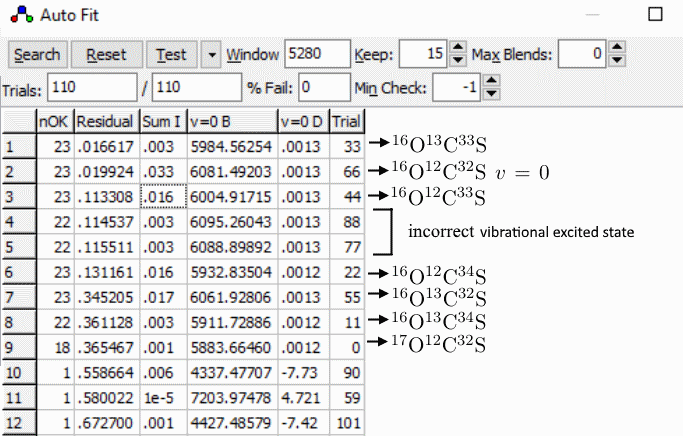
\includegraphics[width=0.85\linewidth]{./pic/ocs_first_try}}
\caption{\small Result of an OCS auto fit.}
\label{fig:ocs_first_try}
\end{figure}

If we decrease $\Delta c$ from its initial guess of $1$ MHz, $n_{OK}$ goes down for all output assignments, until we can't separate correct ones anymore. Also the differences and ratios of $n_{OK}$ between different output rows vary as $\Delta c$ changes. If we increase $\Delta c$ from  its initial guess of $1$ MHz to $3$ MHz, all isotopologues now get all 25 transitions assigned. If we increase it further, the incorrectly treated vibrationally exited transitions also get all transitions assigned (since they obey the same model except for L-doubling, they cannot be separated here). Starting with a value of about $500$ MHz, we cannot separate correct assignments from wrong ones by $n_{OK}$.

We expected that increasing the number of check transitions ($|C|$) and,  simultaneously, increasing $\Delta c$ makes the correct assignments even more separable from the incorrect. And indeed, with $|C| = 40$ and $\Delta c = 10$ MHz, we get almost the same situation as for $|C| = 25$, $\Delta c = 2$ MHz, except that the $n_{OK}$ difference between the right and the wrong has grown to $33$.

We also tried increasing $|C|$ and, simultaneously, adding $H$ to the fit (without changing $\Delta c$). But $H$ is poorly defined from least squares even for $|C| = 40$, and AUTOFIT gives \lq\lq{}rubbish out\rq\rq{}: check transitions are assigned poorly and he Residuals window shows seemingly even larger errors than with only $B$ and $D$ being fitted.

In the third test, we generated spectrum of $\rm ^{16}O^{12}C^{32}S$ $v = 0$ with added random normal errors with $\sigma = 0.1$ MHz to CDMS line positions. %Intuition may suggest that with a $\Delta c = 1$ MHz check transitions would be assigned with $4 \sigma$ confidence or $21--22$ from $23$ check lines. That would be the case if the assignment of search transitions yielded a perfect $M$, so that each check transition would be in the exact theoretical position ($x_0$). 
Since only the 2 fit transitions are fitted in an auto fit, the model gets drastically worse with errors introduced into search transitions. In our case, the higher frequency check transitions get large systematic deviations, but, again, increasing $\Delta c$ allowed to assign all check transitions correctly. The strategy of increasing $\Delta c$ worked also in the next test, where $1000$ random \lq\lq{}weeds\rq\rq{} were added to the spectrum (Fig. \ref{fig:weeds}).

\begin{figure}[h]
\center{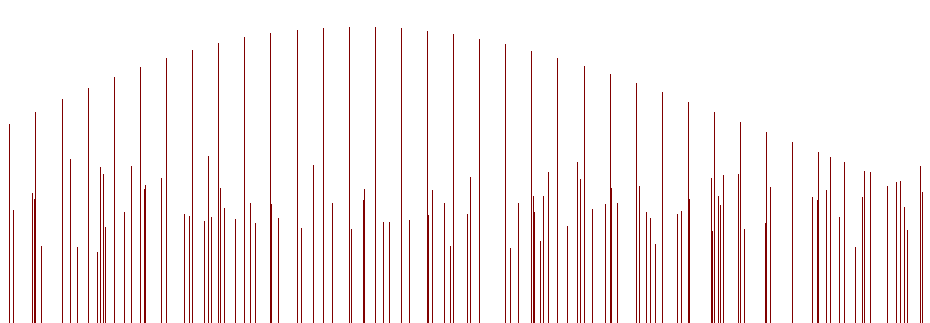
\includegraphics[width=0.85\linewidth]{./pic/weeds}}
\caption{\small A piece of OCS spectrum showing main species in ground vibrational state with additional random \lq\lq{}weed\rq\rq{} lines and random normal noise in line positions.}
\label{fig:weeds}
\end{figure}

The last test combines all the above difficulties -- several species of $\rm OCS$ put together, mixed with \lq\lq{}weeds\rq\rq{} and with added random normal shifts of line positions. With reasonable random shift values ($\sigma = 0.1 MHz$) the correct assignments are still distinguishable in an auto fit with same fit and check transitions as in previous tests (total $40$ transitions), with $B$ and $D$ floated, $\Delta s = 5280$ MHz and upon increasing the check window up to $\Delta c = 60$ MHz. 

As in previous tests, increasing both $\Delta c$ and $|C|$ ultimately yields $n_{OK} = 38$ for correct assignments with a  \lq\lq{}gap\rq\rq{} in $n_{OK}$ between the correct and incorrect assignments in AUTOFIT output. An additional hint particularly for this this case is to look at the similarity of $D$ in output assignments because typically higher order terms vary less then lower order terms between species of a molecule.

But there is also at least one more strategy that can be used: adding another fit transition \emph{without} adding an additional fit parameter. This reduces obs minus calc after the auto fit compared to an auto fit with fewer fit transitions and enlarges the $n_{OK}$ \lq\lq{}gap\rq\rq{}. The main disadvantage -- computation time goes up drastically. %The final output for $3$ fit transitions and $37$ check transitions with a $\Delta c = 35$ MHz is shown in Fig. \ref{fig:ocs_final}.

With all transitions up to 300 GHz assigned, we consider the early stage of assignment complete for this case. Transitions with higher frequencies can be assigned by using the Nearest method -- one only has to worry about floating additional distortions at some point. 

\subsection{Vinyl cyanide}

Vinyl cyanide ($\rm C_2H_3CN$), also known as acrylonitrile or propenenitrile, is an important molecule in space: it has been detected in the Sagittarius B2 star forming region, in dark clouds, circumstellar envelopes, in Titan atmosphere. The molecule is a highly prolate asymmetric top with $\kappa = -0.9798$ for the main isotopic species in its ground vibrational state and two nonzero electric dipole moments $\mu_a = 3.816(3)$ D and $\mu_b = 0.687(8)$ D.  

For a single species and vibrational state of $\rm C_2H_3CN$, 
%For molecules near $\kappa = -1$ the largest rigid rotor constant (typically A) is much larger than the other ones and the spectrum looks almost like a spectrum of a symmetric top.  % TODO: move to introduction
distinct $K$-ladders of $\mu_a$-type lines at different $J$ are the strong features. %The $\mu_a$-type spectra can be actually assigned straightforward, though some different assignments in the middle of a $K-$ladder may need to be tested at early stage.
It is important to float $B$, $C$ and $DJK$ in the initial auto fit, as those constants are the main factors for the mentioned $K$-ladders. 


For the same reason as in the OCS example, we took here artificial mixtures of $\rm C_2H_3CN$ lines from CDMS. In the first test, just the main species was taken as $E$ and one asymmetric top model was created in PGOPHER with only rigid rotational constants $A, B, C$. The initial constant values were derived from true values of a complete parameter list by forcefully setting all distortions and perturbations to zero and then fitting the correct assignment to only $A, B, C$. This gives, in some sense, effective values of $A, B, C$, which mimic ab initio calculation results. %selecting random shifts within $1\%$ of the true value, resembling an ab initio calculations result, where also $1\%$ error is often a fair guess. 

At the early stage of assignment is it reasonable to start again below and around $100$ GHz. We were going to try the brute force approach again and put $\mu_a$-type transitions with $6 \leq J' \leq 14$, with $10\%$ strength cutoff and 140 GHz frequency cutoff (total of 165 transitions), preliminary marked as check transitions, into the Line List.  

%The fit transitions set must have enough  \lq\lq{}diversity\rq\rq{}\todo{what the heck is diversity}  in quantum numbers to minimize the uncertainty after a least squares fit. In respect to that good fit transitions with a fixed total amount may be suggested automatically -- the original AUTOFIT software has this feature. A right thumb approach to this would be to select fit transitions from different K-ladders (i.e. with different $J'$).

Different sets of fit transitions in this test, unlike the simple case of $\rm OCS$, yield considerably different output, although some predicted lines are assigned to the same experimental peaks among several auto fits with different fit transitions. It seems like for this case and more complex cases, visual instruments and human judgment are needed to distinguish \lq\lq{}almost correct\rq\rq{} assignments.

In our case with $\rm 9_{2,7}-8_{2,6}, 9_{1,8}-8_{1,7}, 10_{1,10}-9_{1,9}$ as fit transitions, $2000$ MHz search window and $20$ MHz check window we get a following good and well distinguishable assignment in the first output row. 

The next stage of assignment, the intermediate stage, begins then. Typically it is reasonable to use the Nearest Lines instrument for visualizing the trend of the R-branch lines first, when working in PGOPHER. The Nearest Lines instrument in our case shows a mess when selecting all Kas together, but you can see some trends when selecting individual Kas. There, when viewing a +-1 MHz by 190 GHz window, Ka=1,2,3 have a large curvature, Ka=3,4,5,6 look ok, and Ka >= 8 trends become a large Y axis shift, and that shift is rapidly increasing with increasing Ka, so that for large Kas the correct assignement points are completely out of visibility. 

What also can be noticed is that for some lower Kas the lines are in a sense isolated, so that in a reasonable search window only one experimental peak corresponds to a given transition immediately after AUTOFIT or even before (with only ab initios). These transitons can be assigned right away. But it is not done automatically by now, since the automatic routines are not sure when there is really only one possible candidate, and this decision is left to the human, the humans eye is very good at recognizing patterns. 

Patterns consist of calc transitions repeatedly positioned together at different quantum numbers. There are true patterns and false patterns. Also, already assigned lines from the current species or other isotopologues and vibrational states play a big role. And also the intensity ratios play a big role, thought only locally, and only ratios, not the absolute intensities, for most experiments done, algthough there are experiments which are calibrated to absolute intensities.
 
\subsection{Thiazole}

Thiazole is a ring molecule, well known in infrared, whose vibrationally excited rotation states had not been investigated before. In this work, new analysis methods are applied to their investigation.

At first we do an AUTOFIT run. We want to fit only $B$ and $C$ to the a-type spectrum, but selecting only two fit transitions doesn't give a good result. \todo{Provide a proof for this using vinyl cyanide.} Then we use $3$ fit transitions. 

After selecting the correct result from AUTOFIT output, the middle stage of assignement begins. For the ground vibrational state of the main isotopologue, which has the strongest lines, the middle stage of assignment was quite simple, because in the Nearest Line Plot the trend was immediately visible. That was, however, not the case with v18=1 and even less with v17=1. For these states, some manual search for good assignments and their neighbourhoods were needed.

So it is obvious that an automated procedure should respect already assigned lines from the main species (and others.)
%\begin{figure}[h]
%\center{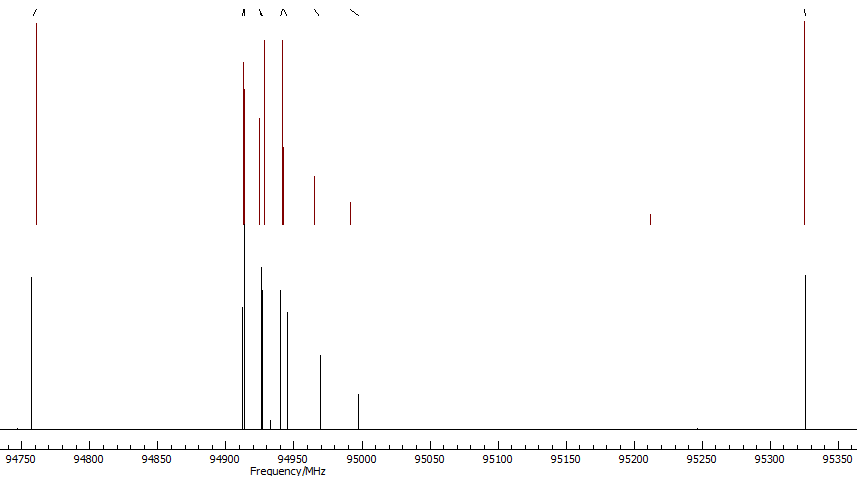
\includegraphics[width=0.85\linewidth]{./pic/vyn_first}}
%\caption{\small The fist step of the early stage assignment of  $\rm C_2H_3CN$ main species (1st test). }
%\label{fig:vyn_first}
%\end{figure}

%The next step would be to add more lines and more fit parameters to the model, possibly re-assigning incorrect assigned lines. Using the Nearest button, we add further $\mu_a$-type lines up to $J' = 19$ with the same Acceptance of $20$ MHz. The residuals in Residuals window are rather uniformly spread with an average of $7.8$ MHz over 300 line positions (most of them are 2-fold degenerate). 


%In the second test, the following mixture was prepared:
% \begin{itemize}
%	\item the main species in ground vibrational state at 100\% CDMS line strength
%	\item 4 isotopologues with a single substituted $\rm ^{13}C$ at 25\% CDMS line strength
%\end{itemize}


%Colin Western in the manual recommends to select $\Delta c$ according to the instrumental resolution. For pure rotational transitions, a better start might be $\Delta s / 10$. It is also good to select $\Delta B$ proportional to $\Delta s$ and inversely proportional to $J$ (because of the formula). Setting $\Delta B$ nonzero saves a lot of calculation time in PGOPHER, about 10 times faster in our case.  

%Observation: when decreasing check window size keeping everything else as it is, fist of all, nOK decreases, but the correct answer is still at the top. But then some wrong assignments can get to the top 20 rows. This supports the idea that when $\Delta c$ is less then the deviation arising from still closed constants, "correct" lines are not assigned, and the right answer competes with wrong ones.

%[Also observation 4, hypothesis 5 and 6. and 7]


\end{document}
